%!TEX TS-program = xelatex
%!TEX encoding = UTF-8 Unicode
%!TEX root = DESpecs.tex


\newpage
\appendix

\section{List of All Tags}
\label{appendix list of all tags}

\newcommand{\eins}{{\fontspec{DejaVu Sans}{①}}}
\newcommand{\zwei}{{\fontspec{DejaVu Sans}{②}}}

\begin{longtable}[l]{@{}llp{4cm}p{4cm}@{}l@{}}
%\begin{tabular}{@{}llll@{}}
section & tag & name & attributes \\[1mm]
\hline \\
\ref{section page breaks} & \xms{pb} & page break &  \attr{pb}{n}, \attr{pb}{rend} & \eins \\
\ref{section page breaks} & \xmlpair*{fw} & running head &\attr{fw}{type="head"}, \attr{pb}{rend}& \eins \\
\\
\ref{textblocks} & \xms{lb} & line break && \\
\ref{section headings} & \xmlpair*{head}& heading & \attr{pb}{rend}& \eins \\
\ref{section paragraphs} & \xmlpair*{p} & paragraph & \attr{pb}{rend}& \eins \\
\ref{section block quotations} & \xmlpair*{quote} & block quotation & \attr{pb}{rend}& \eins \\
\ref{footers} & \xmlpair*{p} & footer & \attr{p}{type="footer"}, \attr{pb}{rend} & \eins \\
\\
\ref{section columns} & \xms{cb} & column & \attr{cb}{n} &  \\
\\
\ref{section tables basic rule} & \xmlpair*{table} & table & \attr{pb}{rend}& \eins \\
\ref{section tables basic rule} & \xmlpair*{row} & table row &\attr{pb}{rend}& \eins \\
\ref{section tables basic rule} & \xmlpair*{cell} & table cell &\attr{cell}{cols}, \attr{cell}{rows}, \attr{pb}{rend}& \eins \\
\\
\ref{section indexes} & \xmlpair*{list} & index &\attr{list}{type="index"}, \attr{pb}{rend}& \eins \\
\ref{section indexes} & \xmlpair*{item} & index entry &\attr{pb}{rend}& \eins \\
\ref{section indexes} & \xmlpair*{ref} & page reference &&  \\
\ref{section tables of contents} & \xmlpair*{list} & table of contents &\attr{list}{type="toc"}, \attr{pb}{rend}& \eins \\
\ref{section tables of contents} & \xmlpair*{item} & table of contents entry & \attr{pb}{rend}& \eins \\
\ref{section tables of contents} & \xmlpair*{ref} & page reference &&  \\
\\
\ref{section marginal notes} &\xmlpair*{note} & marginal note (left) & \attr{note}{place="margin left"}, \attr{pb}{rend} & \eins \\
\ref{section marginal notes} &\xmlpair*{note} & marginal note (right) & \attr{note}{place="margin right"}, \attr{pb}{rend} & \eins \\
\ref{section footnotes} &\xmlpair*{note} & footnote (main text) & \attr{note}{place="bottom"}, \attr{note}{n}, \attr{pb}{rend} & \eins \\
\ref{section anchored comments} &\xmlpair*{note} & anchored comment (left) & \attr{note}{place="margin left"}, \attr{note}{n}, \attr{pb}{rend} & \eins \\
\ref{section anchored comments} &\xmlpair*{note} & anchored comment (right) & \attr{note}{place="margin right"}, \attr{note}{n}, \attr{pb}{rend} & \eins \\
\\
\ref{section figures} & \xms{fig} & simple figure &\attr{figure}{place="here"} & \\
\ref{section figures} & \xmlpair*{fig} & complex figure &\attr{figure}{place="here"} & \\
\ref{section figures} & \xmlpair*{head}  & figure caption & \attr{pb}{rend}& \eins \\
\ref{section figures} & \xmlpair*{ab}& descriptive text in figures & \attr{ab}{type="desc"}, \attr{pb}{rend} & \eins \\
\ref{section figures} & \xmlpair*{ab} &variables in figures & \attr{ab}{type="var"}, \attr{pb}{rend} & \eins \\
\\
\ref{section handwritten notes} & \xms{add} & handwritten note & \attr{add}{rend="handwritten"} \\
\\

% If you have reason to believe that there is a mistake in the text, surround it by  after the element containing the mistake.

\ref{section characters you are unsure about} & \xms{gap} & unreadable text & \\
\ref{section characters you are unsure about} & \xmlpair*{unclear} & uncertain text & \\
\ref{section unknown characters} & \xms{g} & unknown character &\attr{g}{ref} \\
\ref{section obvious mistakes} & \xmlpair*{sic}, \xms{sic} & obvious mistake & \\
\\
\hline \\
\ref{section other diacritics} & §\'q§, etc. & character+diacritic & §' ` ^ " ~ , . = § & §-§ \\
\\

\ref{section italics} & \xmlpair*{hi} & italics & \attr{hi}{rend="emph"} \\
\ref{section bold face} & \xmlpair*{hi} & bold face & \attr{hi}{rend="bold"} \\
\ref{section small caps} & \xmlpair*{hi} & small caps & \attr{hi}{rend="sc"} \\
\ref{section subscript and superscript} &\xmlpair*{hi} & subscript &\attr{hi}{rend="sub"} \\
\ref{section subscript and superscript} &\xmlpair*{hi} & superscript & \attr{hi}{rend="sup"}\\
\ref{section underlines and overlines} &\xmlpair*{hi} & underline &\attr{hi}{rend="ul"} \\
\ref{section underlines and overlines} &\xmlpair*{hi} & overline & \attr{hi}{rend="ol"}\\

\ref{section text in red} &\xmlpair*{hi} & text in red & \attr{hi}{rend="red"}\\
\\
% \ref{section latin ligatures} & §{quo}d§, etc. & resolved ligature & \\
%\ref{section greek ligatures} & §{μεν}§ etc. & Greek ligature & \\
\\
\hline \\
\ref{section fraktur alphabet} & \xmlpair*{hi} & words in Fraktur &\attr{hi}{rend="fr"} \\
\ref{section sperrung} & \xmlpair*{hi} & Sperrung &\attr{hi}{rend="sp"} \\
\ref{section words in roman characters} &\xmlpair*{hi}  & words in roman chars &\attr{hi}{rend="rom"} \\
\\
\hline \\
\ref{section fractions} &\xmlpair*{formula}  & fraction & \\
\ref{section roots} & \xmlpair*{formula}  & root &&  \\
\\
\hline \\
%\end{tabular}
\end{longtable}

\eins \quad This tag may also contain the \attr{several}{rend} attribute with the values §emph§, §bold§, §sc§, §sub§, §sup§, §ul§, §ul§, §red§, §fr§ or §rom§.

% \section{List of All Attributes}
% \label{appendix list of all attributes}

% \begin{longtable}[l]{@{}lll@{}l@{}}
%  Tag & attributes & values & example \\[1mm]
% \hline \\

% % rend emph fr

% \xms{pb} &  \attr{pb}{n} & page number & \xmex{<pb n="6"/>}\\
% \xml{fw} & \attr{fw}{type="head"} & "head" & \xmex{<fw type="head">GEOMET. ELEMENT. EVCLIDIS</fw>}\\
% \xmlpair*{p} & \attr{p}{type="footer"}, \attr{p}{rend="emph"} &\attr{p}{type="footer"}, \attr{p}{rend="emph"} &\\
% \xms{cb} &  \attr{cb}{n}  & \xmex{<cb n="1"/>} & \\
%  & \attr{several}{rend} && \\
% \xmlpair*{cell} & \attr{cell}{rows}, \attr{cell}{cols} &&\\

% For \attr{table}{rend=''emph''} see \sect{section italics}.

% A note in the  margins is marked by \xmlpair{note} and the attribute \attr{note}{place} with the value `margin left' or `margin right', depending on the side the note is on. Type the marginal note on separate lines, starting after the line it is closest to.
% Footnotes are marked by \xmlpair{note} and the attribute \attr{note}{place} with the value `bottom'. Type the footnote at the place of the footnote symbol or number and record that number in the \attr{note}{n} attribute.
% An anchored note in the margins is marked by \xmlpair{note} and the attribute \attr{note}{place} with the value `margin left' or `margin right', depending on the side the note is on. In addition, the anchor symbol is treated like a footnote symbol, i.e. it is marked by the attribute \attr{note}{n}.
% Where a figure occurs in the text, type \xmsatt{figure}{place}{here} on a separate line. If you can identify a caption of the figure, mark it with \xmlpair{head}. Additional text that describes parts of the figure is marked by the \xml{ab} element and the attribute \attr{ab}{type="desc"}. Use another \xml{ab} element with the attribute \attr{ab}{type="var"} to record variable names and numbers.
% If the character is indeed unknown: Assign the number §001§ to the first unknown character, §002§ to the second unknown character, and so on and record them in the \attr{g}{ref} attribute of the \xms{g} tag, prefixed with the character §#§ . Do not assign the same number twice. Use this number to type the unknown character. Always use the same number if the same unknown character occurs again.
% If you have reason to believe that there is a mistake in the text, surround it by \xmlpair{sic}, or if the mistake is encoded in an attribute, use a milestone tag, \xms{sic} after the element containing the mistake.
% Use the element \xmlatt{hi}{rend}{emph} to mark words or whole lines in italics. Encode only up to a few lines of text this way. A whole paragraph in italics is marked by the \attr{p}{rend="emph"} in the \xml{p} tag. Also, be careful not to include punctuation marks.
%   Within a larger \attr{p}{rend="emph"} structure like paragraph, table or page you can use \xmlpatt{hi}{rend}{emph} to mark single words in upright type (see §_THEON_§ in example 2 in \sect{section figures}).
% Mark single words or lines in Fraktur by \xmlpatt{hi}{rend}{fr}. Mark paragraphs in Fraktur by \xml{p rend="fr"}. Mark whole pages in Fraktur by \xms{pb rend="fr"}. If the whole book is in Fraktur or mostly in Fraktur, add the \attr{body}{rend="fr"} attribute to the \xml{body} tag. Type letters in Fraktur as normal roman characters.
% \end{longtable}


\newpage

\section{List of All Symbols}
\label{appendix list of all symbols}

% also: table of characters to be typed directly? MH: no
% if there is a “Symbols” section, will this appendix be unnecessary? MH: hier lassen!

\begin{tabelle}[ 1: \, common footnote symbols (from \sect{section footnotes})]
\begin{tabular}{@{}lc@{\, }c@{\, }c@{\, }c@{\, }c@{\, }c@{\, }c} \\
symbol & * & † & ‡ & \§ & ‖ & ¶ \\[2mm]
Unicode &  \xs{U+002A} & \xs{U+2020} & \xs{U+2021} &\xs{U+00A7} & \xs{U+2016} & \xs{U+00B6} \\
\end{tabular}
\end{tabelle}

\vspace{5mm}

\begin{tabelle}[ 2: \, dashes (see \sect{section dashes})]
\begin{tabular}{@{}lc@{\, }c@{\, }c@{\, }c@{\, }c@{\, }c} \\
symbol & - & – & — \\[2mm]
Unicode & \xs{U+002D} & \xs{U+2013} & \xs{U+2014} & \\
\end{tabular}
\end{tabelle}

\vspace{5mm}

\begin{tabelle}[ 3: \, common mathematical symbols (from \sect{section mathematical symbols})]
\begin{tabular}{@{}lc@{\, }c@{\, }c@{\, }c@{\, }c@{\, }c@{\, }c@{\, }c@{\, }c@{\, }c} \\
symbol & ′ & ″ & ± & \unicode{∴} & ° & ∞ & · & ÷ & √ & Ŗ \\[2mm]
Unicode & \xs{U+2032} & \xs{U+2033} & \xs{U+00B1} & \xs{U+2234} & \xs{U+00B0} & \xs{U+221E} & \xs{U+00F7} & \xs{U+00B7} & \xs{U+221A} & \xs{U+0156} \\[2mm]
\end{tabular}
\end{tabelle}

\vspace{5mm}

\begin{tabelle}[ 4: \, planet symbols (from \sect{section astronomy})]
\begin{tabular}{@{}lc@{\, }c@{\, }c@{\, }c@{\, }c@{\, }c@{\, }c@{\, }c@{\, }c@{\, }c} \\
symbol & \unicode{☿} & \unicode{♀} & \unicode{♁} & \unicode{♂} & \unicode{♃} & \unicode{♄} \\[2mm]
Unicode & \xs{U+263F} & \xs{U+2640} & \xs{U+2641} & \xs{U+2642} & \xs{U+2643} & \xs{U+2644} \\[2mm]
\end{tabular}
\end{tabelle}

\vspace{5mm}

\begin{tabelle}[ 5: \, zodiac symbols (from \sect{section astronomy})]
\begin{tabular}{@{}lc@{\, }c@{\, }c@{\, }c@{\, }c@{\, }c} \\
symbol & \unicode{♈} & \unicode{♉} & \unicode{♊} & \unicode{♋} & \unicode{♌} & \unicode{♍} \\[2mm]
Unicode & \xs{U+2648} & \xs{U+2649} & \xs{U+264A} & \xs{U+264B} & \xs{U+264C} & \xs{U+264D} \\[4mm]
symbol & \unicode{♎} & \unicode{♏} & \unicode{♐} & \unicode{♑} & \unicode{♒} & \unicode{♓} \\[2mm]
Unicode & \xs{U+264E} & \xs{U+264F} & \xs{U+2650} & \xs{U+2651} & \xs{U+2652} & \xs{U+2653} \\[2mm]
\end{tabular}
\end{tabelle}


\vspace{5mm}

\begin{tabelle}[ 6: \, technical symbols (from \sect{section technical symbols})]
\begin{tabular}{@{}lc@{\, }c@{\, }c@{\, }c@{\, }c@{\, }c@{\, }c@{\, }c@{\, }c@{\, }c} \\
symbol & \unicode{℞} \\[2mm]
Unicode & \xs{U+211E} \\[2mm]
\end{tabular}
\end{tabelle}


\newpage
\section{Example Transcriptions}

\tocspace
\subsection{Latin Example}
\label{Structural markup general example}

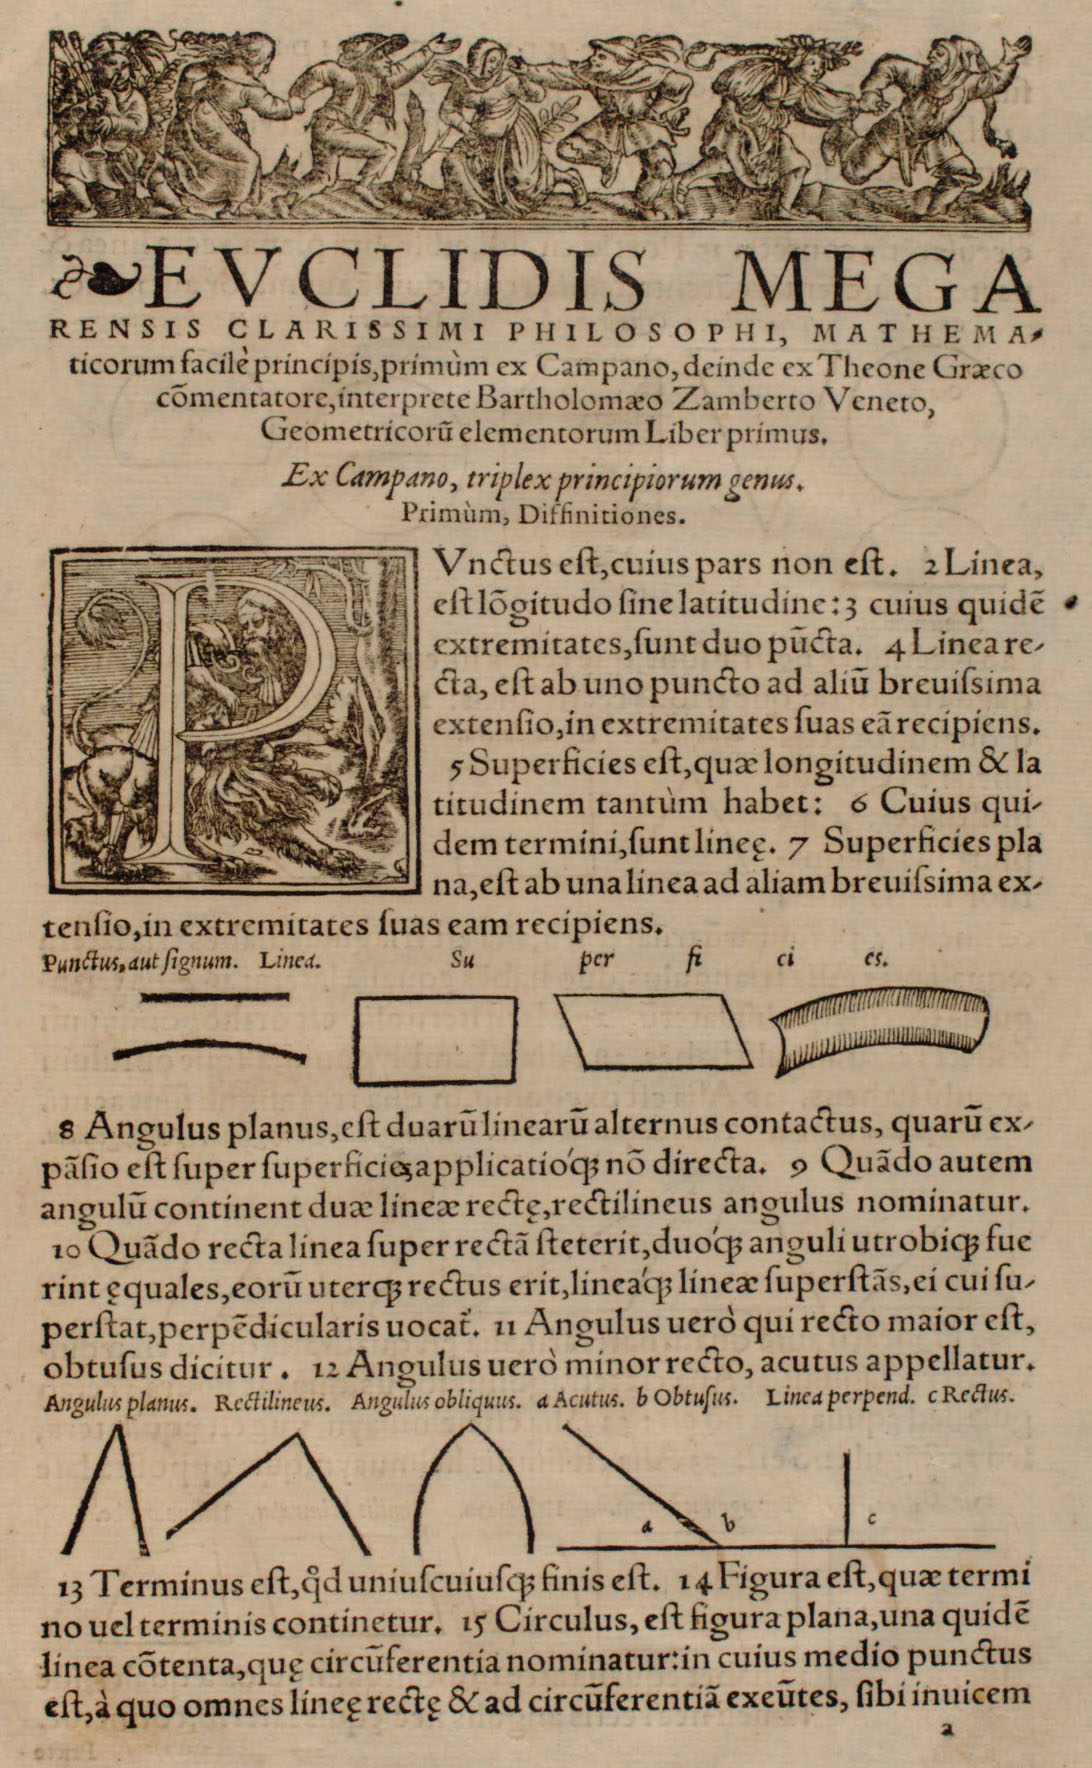
\includegraphics[height=22cm]{euclid_wholepage_3}
\clearpage

\begin{typeLatin}
\bold{<pb/>} \\
\bold{<figure place="here"/>} \\
\bold{<figure place="here"/>} \\
\bold{<head>}EVCLIDIS MEGA\bold{<lb/>} \\
RENSIS CLARISSIMI PHILOSOPHI, MATHEMA-\bold{<lb/>} \\
ticorum facilè principis, primùm ex Campano, deinde ex Theone Grӕco\bold{<lb/>} \\
cõmentatore, interprete Bartholomӕo Zamberto Veneto,\bold{<lb/>} \\
Geometricorũ elementorum Liber primus.\bold{</head>} \\
\bold{<head rend="emph">}Ex Campano, triplex principiorum genus.\textbf{</head>} \\
\bold{<head>}Primùm, Diffinitiones.\bold{</head>} \\
\bold{<p>}PVnctus eſt, cuius pars non eſt. 2 Linea,\bold{<lb/>} \\
eſt lõgitudo ſine latitudine: 3 cuius quidẽ\bold{<lb/>} \\
extremitates, ſunt duo p\bs\tld{}ucta. 4 Linea re-\bold{<lb/>} \\
cta, eſt ab uno puncto ad ali\bs\tld{}u breuiſsima\bold{<lb/>} \\
extenſio, in extremitates ſuas eã recipiens.\bold{<lb/>} \\
5 Superficies eſt, quæ longitudinem &amp; la\bold{<lb/>} \\
titudinem tantùm habet: 6 Cuius qui-\bold{<lb/>} \\
dem termini, ſunt line\li{ae}. 7 Superficies pla\bold{<lb/>} \\
na, eſt ab una linea ad aliam breuiſsima ex-\bold{<lb/>} \\
tenſio, in extremitates ſuas eam recipiens.\bold{</p>}\\
\bold{<figure place="here">}\\
\bold{<head rend="emph">}\bold{<hi rend="emph">}P\bold{</hi>}unctus, aut ſignum. \lwr\bold{<hi rend="emph">}L\bold{</hi>}inea.\bold{</head>}\\
\bold{</figure>}\\
\bold{<figure place="here">}\\
\bold{<head rend="emph">}Su per fi ci es.\bold{</head>}\\
\bold{</figure>}\\
\bold{<p>}8 Angulus planus, eſt duar\bs\tld{}u linear\bs\tld{}u alternus contactus, quar\bs\tld{}u ex-\bold{<lb/>} \\
pãſio eſt ſuper ſuperficies,\bold{<unclear/>} applicatio´\li{que} nõ directa. 9 Quãdo autem\bold{<lb/>} \\
angul\bs\tld{}u continent duæ lineæ rect\li{ae}, rectilineus angulus nominatur.\bold{<lb/>} \\
10 Quãdo recta linea ſuper rectã ſteterit, duo´\li{que} anguli utrobi\li{que} fue\bold{<lb/>} \\
rint \li{ae}quales, eor\bs\tld{}u uter\li{que} rectus erit, linea´\li{que} lineæ ſuperſtãs,\lwr ei cui ſu-\bold{<lb/>} \\
perſtat, perp\bs\tld{}edicularis uoca\li{tur}. 11 Angulus uerò qui recto maior eſt,\bold{<lb/>} \\
obtuſus dicitur. 12 Angulus uerò minor recto, acutus appellatur.\bold{</p>}\\
\bold{<figure place="here">}\\
\bold{<head rend="emph">}\bold{<hi rend="emph">}A\bold{</hi>}ngulus planus.\bold{</head>}\\
\bold{</figure>}\\
\bold{<figure place="here">}\\
\bold{<head rend="emph">}\bold{<hi rend="emph">}R\bold{</hi>}ectilineus.\bold{</head>}\\
\bold{</figure>}\\
\bold{<figure place="here">}\\
\bold{<head rend="emph">}\bold{<hi rend="emph">}A\bold{</hi>}ngulus obliquus.\bold{</head>}\\
\bold{</figure>}\\
\bold{<figure place="here">}\\
\bold{<head rend="emph">}Linea perpend.\bold{</head>}\\
\bold{<ab type="desc" rend="emph">}a Acutus.\bold{</ab>}\\
\bold{<ab type="desc" rend="emph">}b Obtuſus.\bold{</ab>}\\
\bold{<ab type="desc" rend="emph">}c Rectus.\bold{</ab>}\\
\bold{<ab type="var" rend="emph">}a b c\bold{</ab>}\\
\bold{</figure>}\\
\bold{<p>}13 Terminus eſt, \li{quo}d uniuſcuiuſ\li{que} finis eſt. 14 Figura eſt, quæ termi\bold{<lb/>} \\
no uel terminis continetur. 15 Circulus, eſt figura plana, una quid\bs\tld{}e\bold{<lb/>} \\
linea cõtenta, qu\li{ae} circ\bs\tld{}uferentia nominatur: in cuius medio punctus\bold{<lb/>} \\
eſt, à quo omnes line\li{ae} rect\li{ae} &amp; ad circ\bs\tld{}uferentiã exe\bs\tld{}utes,\lwr ſibi inuicem\bold{<lb/>} \\
\end{typeLatin}

\begin{note}
The character bottom right is the catchword, it is not the page number of this page. The closing §</p>§ of the last paragraph is on the next page.

%The typesetter used the page number of the next page as a catchword, i.e. it is not the page number of this page. The closing §</p>§ of the last paragraph is on the next page.
\end{note}

\vfill


\tocspace
\subsection{Greek Example}
\label{section greek example}

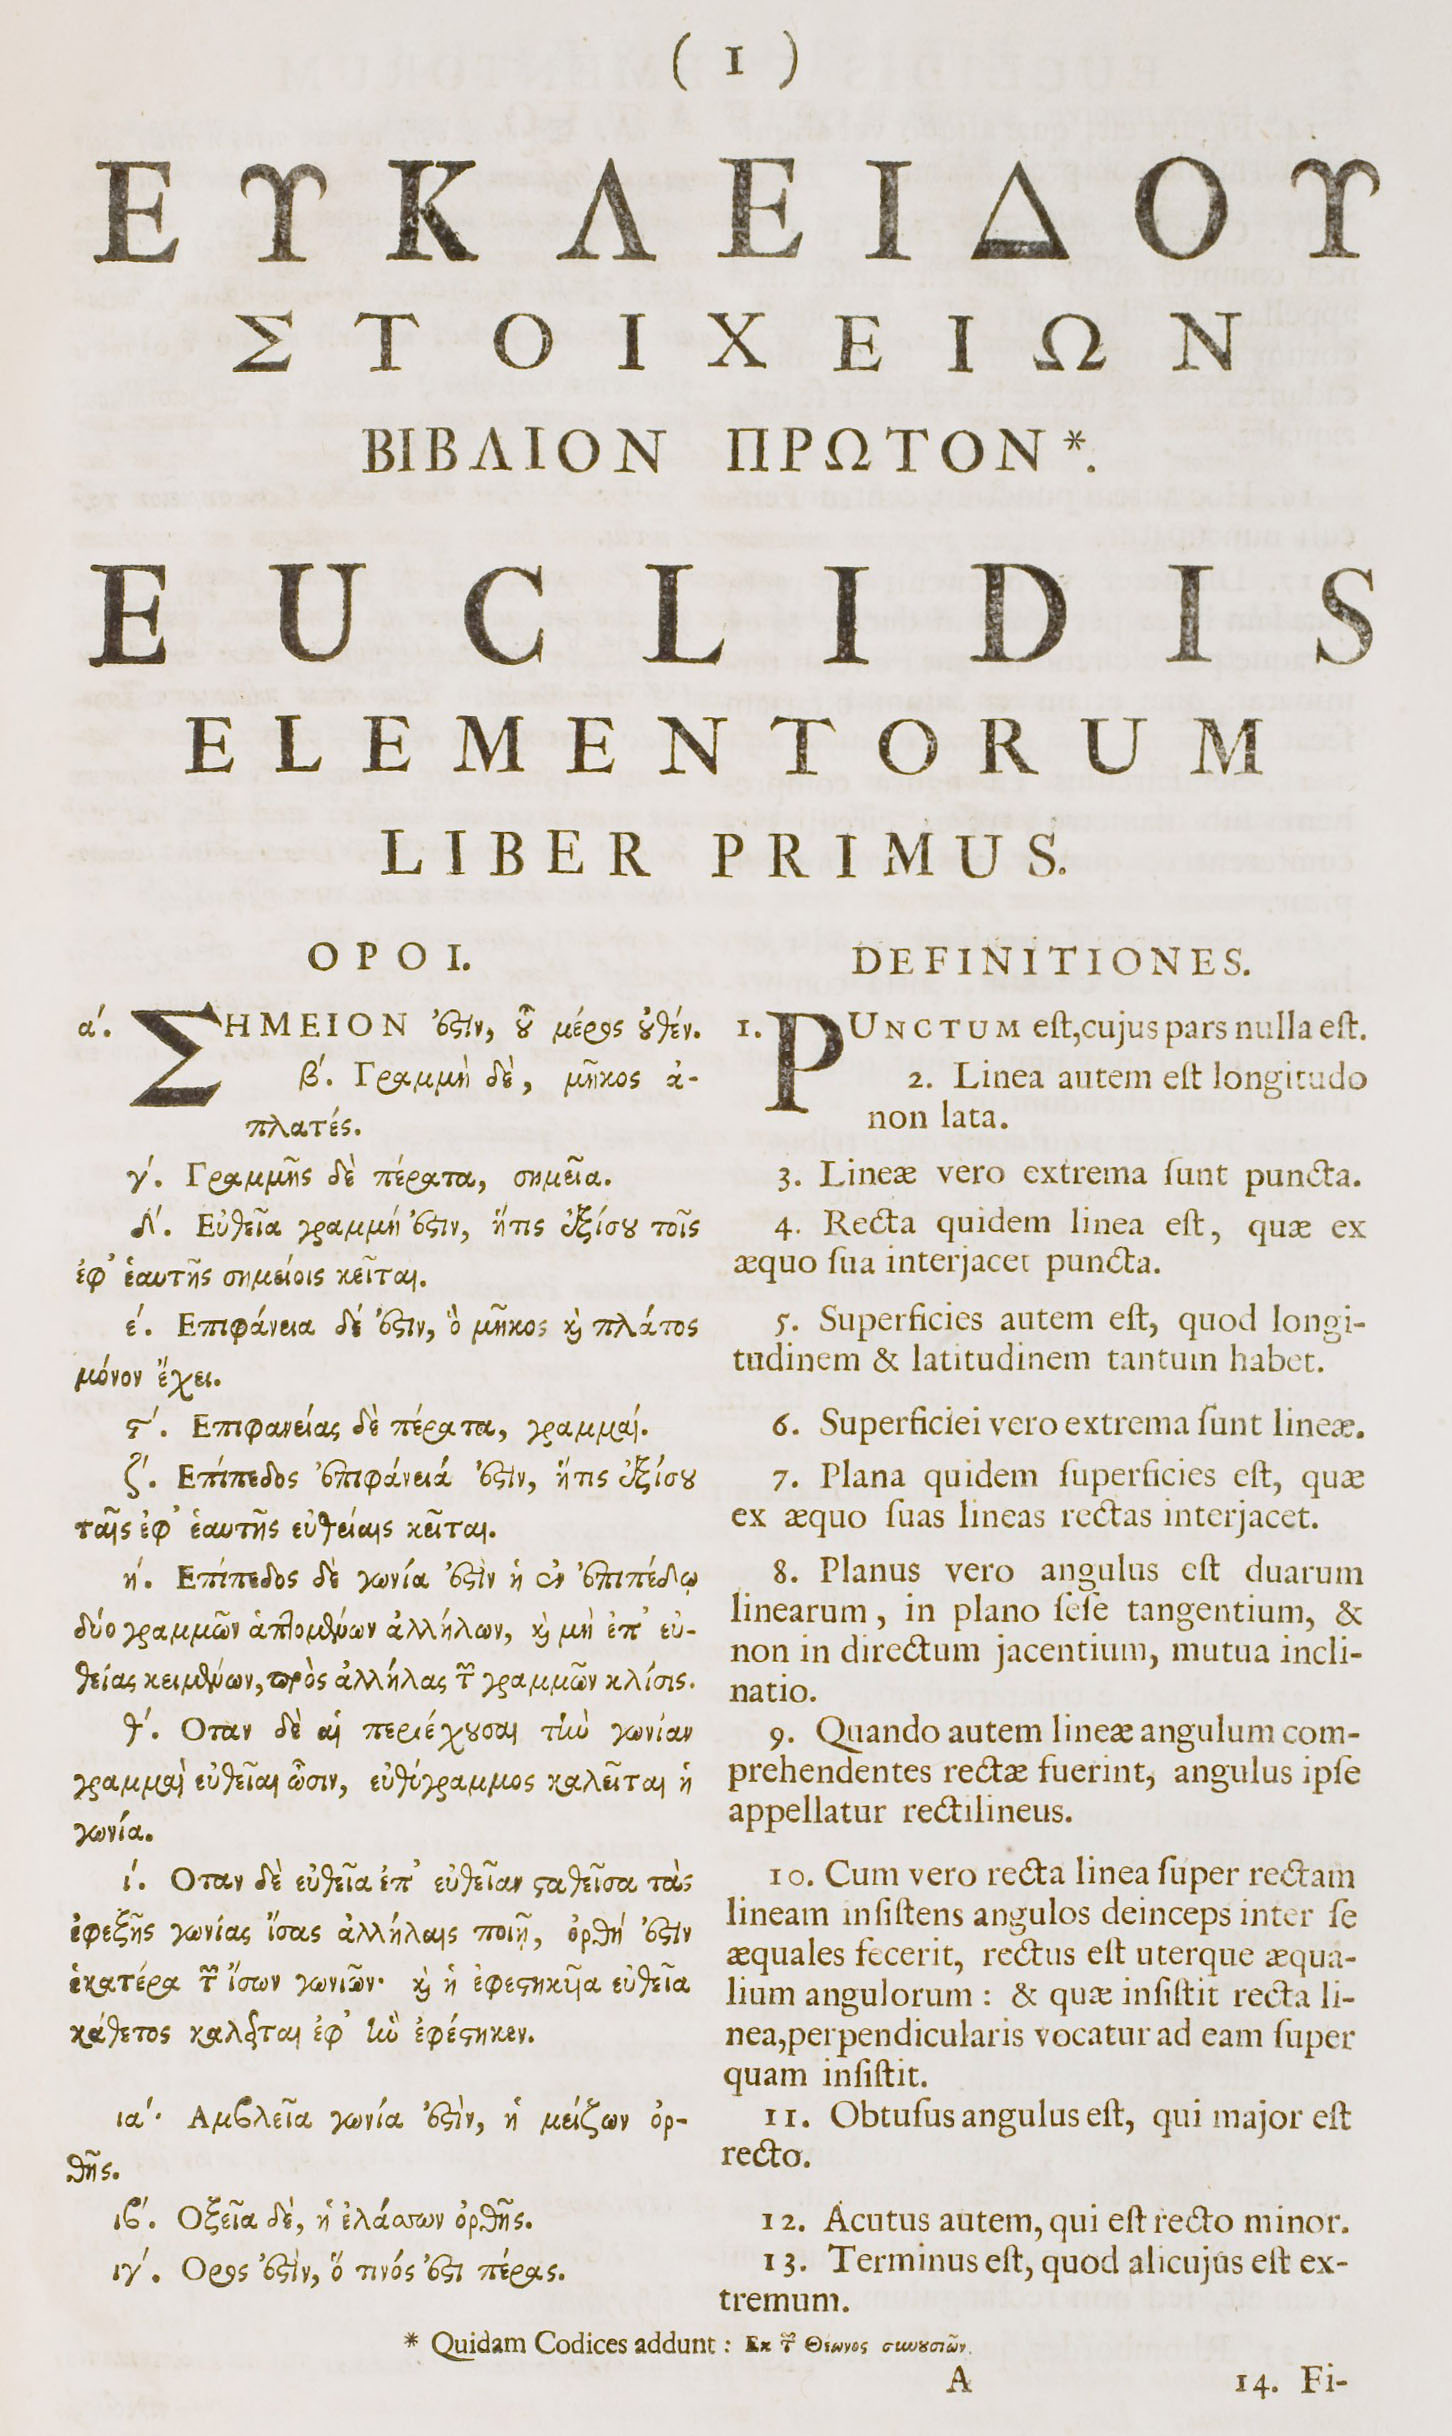
\includegraphics[height=23cm]{euklid_gr_lat_p25_2}
\clearpage

\begin{typeLatin}
\bold{<pb n="1"/>} \\
\bold{<head>}ΕΥΚΛΕΙΔΟΥ\bold{<lb/>} \\
ΣΤΟΙΧΕΙΩΝ\bold{<lb/>} \\
ΒΙΒΛΙΟΝ ΠΡΩΤΟΝ \bold{<note place="bottom" n="*">}Quidam Codices addunt: Εκ \li{τῶν} Θέωνος\lwr σ\li{υν}\li{ου}\li{σι}ῶν.\bold{</note>}.\bold{</head>} \\
\bold{<head>}EUCLIDIS\bold{<lb/>} \\
ELEMENTORUM\bold{<lb/>} \\
LIBER PRIMUS.\bold{</head>}\\
\bold{<cb n="1"/>}\\
\bold{<head>}ΟΡΟΙ.\bold{</head>}\\
\bold{<p>}α'. ΣΗΜΕΙΟΝ \li{ἐστι}ν, \li{οὗ} μέ\li{ρο}ς \li{οὐ}\li{θέ}ν.\bold{</p>} \\
\bold{<p>}β'. Γ\li{ρα}μ\li{μὴ} \li{δὲ}, \li{μῆ}\li{κο}ς ἀ- \bold{<lb/>} \\
\li{πλ}ατές.\bold{</p>} \\
\bold{<p>}γ'. Γ\li{ρα}μ\li{μῆ}ς \li{δὲ} \li{πέ}\li{ρα}\li{τα}, \li{ση}μ\li{εῖ}α.\bold{</p>} \\
\bold{<p>}δ'. Εὐ\li{θε}ῖα \li{γρ}αμ\li{μή} \li{ἐστι}ν, ἥ\li{τι}ς \li{ἐξ}ίσ\li{ου} \li{το}ῖς \bold{<lb/>} \\
ἐφ' ἑ\li{αυ}τῆς \li{ση}μ\li{εί}οις \li{κε}ῖτ\li{αι}.\bold{</p>} \\
\bold{<p>}ε'. Ε\li{πι}φάν\li{ει}α \li{δέ} \li{ἐστι}ν, ὃ \li{μῆ}\li{κο}ς \li{καὶ} \li{πλ}ά\li{το}ς \bold{<lb/>} \\
\li{μό}νον ἔχ\li{ει}.\bold{</p>} \\
\bold{<p>}ϛ'. Ε\li{πι}φ\li{αν}\li{εί}\li{ας} \li{δὲ} \li{πέ}\li{ρα}\li{τα}, \li{γρ}αμμ\li{αί}.\bold{</p>} \\
\bold{<p>}ζ'. Ε\li{πί}\li{πε}\li{δο}ς \li{ἐπι}φάν\li{ει}ά \li{ἐστι}ν, ἥ\li{τι}ς \li{ἐξ}ίσ\li{ου} \bold{<lb/>} \\
τ\li{αῖ}ς ἐφ' ἑ\li{αυ}\li{τῆ}ς εὐθ\li{εί}\li{αι}ς κ\li{εῖ}τ\li{αι}.\bold{</p>} \\
\bold{<p>}η'. Ε\li{πί}\li{πε}\li{δο}ς \li{δὲ} \li{γω}νία \li{ἐστὶ}ν ἡ \li{ἐν} \li{ἐπι}\li{πέδ}ῳ \bold{<lb/>} \\
\li{δύ}ο \li{γρ}αμ\li{μῶ}ν ἁ\li{πτ}ο\li{μέν}ων ἀ\li{λλ}ήλων, \li{καὶ} \li{μὴ} ἐπ' εὐ- \bold{<lb/>} \\
\li{θε}ί\li{ας} κ\li{ει}\li{μέν}ων, \li{πρ}ὸς ἀ\li{λλ}ήλ\li{ας} \li{τῶν} \li{γρ}αμμῶν κλί\li{σι}ς.\bold{</p>} \\
\bold{<p>}θ'. Ο\li{τα}ν \li{δὲ} \li{αἱ} \li{πε}\li{ρι}έχ\li{ου}\li{σαι} \li{τὴν} \li{γω}νί\li{αν} \bold{<lb/>} \\
\li{γρ}αμ\li{μαὶ} εὐ\li{θε}ῖ\li{αι} ὦ\li{σι}ν, εὐ\li{θύ}\li{γρ}αμ\li{μο}ς \li{κα}λ\li{εῖ}τ\li{αι} ἡ \bold{<lb/>} \\
\li{γω}νία.\bold{</p>} \\
\bold{<p>}ι'. Ο\li{τα}ν \li{δὲ} εὐ\li{θε}ῖα ἐπ' εὐ\li{θε}ῖ\li{αν} \li{στα}\li{θε}ῖ\li{σα} \li{τὰ}ς \bold{<lb/>} \\
ἐφεξῆς \li{γω}νί\li{ας} ἴ\li{σα}ς ἀ\li{λλ}ήλ\li{αι}ς \li{πο}ιῇ, ὀρ\li{θή} \li{ἐστι}ν \bold{<lb/>} \\
ἑ\li{κα}τέ\li{ρα} \li{τῶν} ἴ\li{σω}ν \li{γω}νιῶν· \li{καὶ} ἡ ἐφε\li{στη}κ\li{υῖ}α εὐ\li{θε}ῖα \bold{<lb/>} \\
\li{κά}\li{θε}\li{το}ς \li{κα}λ\li{εῖ}τ\li{αι} ἐφ' \li{ἣν} ἐφέ\li{στη}\li{κε}ν.\bold{</p>} \\
\bold{<p>}ια'. Αμβλεῖα \li{γω}νία \li{ἐστὶ}ν, ἡ μ\li{εῖ}ζων ὀρ- \bold{<lb/>} \\
\li{θῆ}ς.\bold{</p>} \\
\bold{<p>}ιβ'. Οξεῖα \li{δὲ}, ἡ ἐλά\li{σσω}ν ὀρ\li{θῆ}ς.\bold{</p>} \\
\bold{<p>}ιγ'. Ο\li{ρο}ς \li{ἐστὶ}ν, ὅ \li{τι}νός \li{ἐστι} \li{πέ}\li{ρα}ς.\bold{</p>} \\
\bold{<cb n="2"/>}\\
\bold{<head>}DEFINITIONES.\bold{</head>}\\
\bold{<p>}1. PU\bold{<hi rend="sc">}NCTUM\bold{</hi>} eſt, cujus pars nulla eſt.\bold{</p>}\\
\bold{<p>}2. Linea autem eſt longitudo\bold{<lb/>} \\
non lata.\bold{</p>}\\
\bold{<p>}3. Lineæ vero extrema ſunt puncta.\bold{</p>}\\
\bold{<p>}4. Recta quidem linea eſt, quæ ex\bold{<lb/>} \\
æquo ſua interjacet puncta.\bold{</p>}\\
\bold{<p>}5. Superficies autem eſt, quod longi-\bold{<lb/>} \\
tudinem &amp; latitudinem tantum habet.\bold{</p>}\\
\bold{<p>}6. Superficiei vero extrema ſunt lineæ.\bold{</p>}\\
\\\untranscribedText \\ \\
\bold{<p>}12. Acutus autem, qui eſt recto minor.\bold{</p>}\\
\bold{<p>}13. Terminus eſt, quod alicujus eſt ex-\bold{<lb/>} \\
tremum.\bold{</p>}\\
\end{typeLatin}

%\bold{<p>}7. Plana quidem ſuperficies eſt, quæ\\
%ex æquo ſuas lineas rectas interjacet.\bold{</p>}\\
%\bold{<p>}8. Planus vero angulus eſt duarum\\
%linearum, in plano ſeſe tangentium, &\\
%non in directum jacentium, mutua incli-\\
%natio.\bold{</p>}\\
%\bold{<p>}9. Quando autem lineæ angulum com-\\
%prehendentes rectæ fuerint, angulus ipſe\\
%appellatur rectilineus.\bold{</p>}\\
%\bold{<p>}10. Cum vero recta linea ſuper rectam\\
%lineam inſiſtens angulos deinceps inter ſe\\
%æquales fecerit, rectus eſt uterque æqua-\\
%lium angulorum: & quæ inſiſtit recta li-\\
%nea, perpendicularis vocatur ad eam ſuper\\
%quam inſiſtit.\bold{</p>}\\
%\bold{<p>}11. Obtuſus angulus eſt, qui major eſt\\
%recto.\bold{</p>}\\

\begin{note}
%The character §ϛ§, which stands for the number 6, should be typed as U+03DB (Greek small letter stigma).
The character §ϛ§, which occurs only once on this page (in §<p>ϛ'§) and stands for the number 6, is not an end-sigma §ς§, but a stigma. It should be typed as U+03DB (Greek small letter stigma).
%The character §ϛ§, which occurs only once on this page (in §<p>ϛ'§), stands for the number 6. It is not an end-sigma §ς§ and should be typed as U+03DB (Greek small letter stigma).
\end{note}
